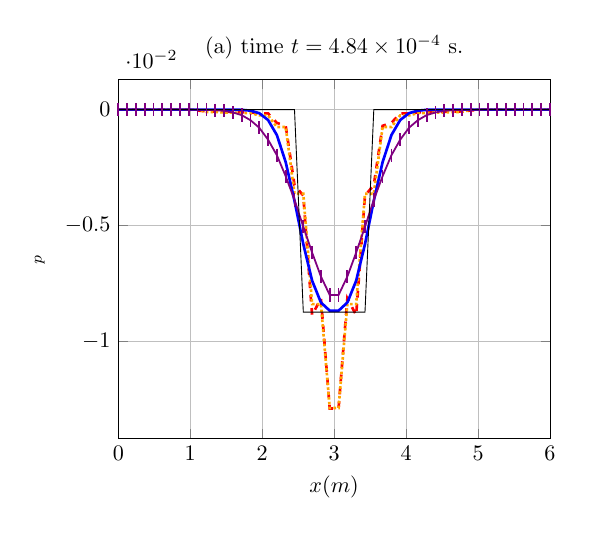
\begin{tikzpicture}[scale=0.8]
\begin{axis}[xlabel=$x (m)$,ylabel=$\eps^p$,ymajorgrids=true,xmajorgrids=true,legend pos=outer north east,title={(a) time $t = 4.84\times 10^{-4} $ s.},xmin=0.,xmax=6.]
\addplot[Red,very thick,mark=none,dashed,mark size=3pt] coordinates {(0.0,0.0) (0.12244897959183673,0.0) (0.24489795918367346,0.0) (0.36734693877551017,0.0) (0.4897959183673469,0.0) (0.6122448979591837,0.0) (0.7346938775510203,0.0) (0.8571428571428571,0.0) (0.9795918367346939,0.0) (1.1020408163265305,-3.791590211516079e-05) (1.2244897959183674,-7.70866275263142e-05) (1.346938775510204,-8.497586707829323e-05) (1.4693877551020407,-9.030872437715389e-05) (1.5918367346938775,-9.742060457186303e-05) (1.7142857142857142,-0.00011777294632526181) (1.836734693877551,-0.00011877997120884317) (1.9591836734693877,-0.00017229593911894644) (2.0816326530612246,-0.0001625095927714705) (2.204081632653061,-0.0005721718460187986) (2.326530612244898,-0.0006980928227095806) (2.4489795918367347,-0.003255684770391246) (2.571428571428571,-0.003703854150331533) (2.693877551020408,-0.008855536230217072) (2.816326530612245,-0.008134161982050364) (2.9387755102040813,-0.012877303196726952) (3.061224489795918,-0.012877303196726607) (3.183673469387755,-0.008134161982050527) (3.306122448979592,-0.008855536230216924) (3.4285714285714284,-0.00370385415033155) (3.5510204081632653,-0.0032556847703911866) (3.673469387755102,-0.0006980928227095723) (3.7959183673469385,-0.0005721718460187898) (3.9183673469387754,-0.0001625095927714674) (4.040816326530612,-0.00017229593911894956) (4.163265306122449,-0.00011877997120884148) (4.285714285714286,-0.00011777294632525957) (4.408163265306122,-9.74206045718636e-05) (4.530612244897959,-9.030872437715303e-05) (4.653061224489796,-8.497586707829776e-05) (4.775510204081632,-7.708662752631704e-05) (4.8979591836734695,-3.791590211516108e-05) (5.020408163265306,0.0) (5.142857142857142,0.0) (5.26530612244898,0.0) (5.387755102040816,0.0) (5.5102040816326525,0.0) (5.63265306122449,0.0) (5.755102040816326,0.0) (5.877551020408163,0.0) (6.0,0.0) };
\addplot[Orange,very thick,mark=none,densely dotted,mark size=3pt] coordinates {(0.0,0.0) (0.12244897959183673,0.0) (0.24489795918367346,0.0) (0.36734693877551017,0.0) (0.4897959183673469,0.0) (0.6122448979591837,0.0) (0.7346938775510203,0.0) (0.8571428571428571,0.0) (0.9795918367346939,0.0) (1.1020408163265305,0.0) (1.2244897959183674,-0.00010125340605535082) (1.346938775510204,-0.00010125340605535564) (1.4693877551020407,-0.00012349527304735526) (1.5918367346938775,-0.00012349527304735214) (1.7142857142857142,-0.0001510249264983643) (1.836734693877551,-0.0001510249264983569) (1.9591836734693877,-0.0002468617206963456) (2.0816326530612246,-0.00024686172069637857) (2.204081632653061,-0.0007504349417450695) (2.326530612244898,-0.0007504349417451243) (2.4489795918367347,-0.0036281593420660124) (2.571428571428571,-0.003628159342065948) (2.693877551020408,-0.008380076410022513) (2.816326530612245,-0.008380076410022256) (2.9387755102040813,-0.012853848358106693) (3.061224489795918,-0.0128538483581062) (3.183673469387755,-0.008380076410022525) (3.306122448979592,-0.008380076410022235) (3.4285714285714284,-0.003628159342066054) (3.5510204081632653,-0.00362815934206591) (3.673469387755102,-0.000750434941745111) (3.7959183673469385,-0.0007504349417450832) (3.9183673469387754,-0.00024686172069633743) (4.040816326530612,-0.00024686172069637695) (4.163265306122449,-0.00015102492649834897) (4.285714285714286,-0.0001510249264983674) (4.408163265306122,-0.00012349527304735949) (4.530612244897959,-0.00012349527304735412) (4.653061224489796,-0.00010125340605534598) (4.775510204081632,-0.00010125340605535762) (4.8979591836734695,0.0) (5.020408163265306,0.0) (5.142857142857142,0.0) (5.26530612244898,0.0) (5.387755102040816,0.0) (5.5102040816326525,0.0) (5.63265306122449,0.0) (5.755102040816326,0.0) (5.877551020408163,0.0) (6.0,0.0) };
\addplot[Blue,very thick,mark=none,solid,mark size=3pt] coordinates {(0.0,0.0) (0.12244897959183673,0.0) (0.24489795918367346,0.0) (0.36734693877551017,0.0) (0.4897959183673469,0.0) (0.6122448979591837,-5.222502208891369e-16) (0.7346938775510203,-3.801924841744559e-14) (0.8571428571428571,-1.3141666139875138e-12) (0.9795918367346939,-2.8745591924304055e-11) (1.1020408163265305,-4.464150179000128e-10) (1.2244897959183674,-5.23467841943105e-09) (1.346938775510204,-4.812046858639944e-08) (1.4693877551020407,-3.554036475964955e-07) (1.5918367346938775,-2.1443096765697003e-06) (1.7142857142857142,-1.0689498023182154e-05) (1.836734693877551,-4.436466051051049e-05) (1.9591836734693877,-0.00015404085928397946) (2.0816326530612246,-0.00044873332231471766) (2.204081632653061,-0.0010984305872627827) (2.326530612244898,-0.0022622254025038953) (2.4489795918367347,-0.003929978610103271) (2.571428571428571,-0.005797119893456445) (2.693877551020408,-0.007371043418348148) (2.816326530612245,-0.008310826779347521) (2.9387755102040813,-0.00866523151909913) (3.061224489795918,-0.008665231519099129) (3.183673469387755,-0.008310826779347523) (3.306122448979592,-0.007371043418348151) (3.4285714285714284,-0.0057971198934564485) (3.5510204081632653,-0.003929978610103277) (3.673469387755102,-0.002262225402503906) (3.7959183673469385,-0.0010984305872627934) (3.9183673469387754,-0.0004487333223147267) (4.040816326530612,-0.00015404085928398656) (4.163265306122449,-4.4364660510512195e-05) (4.285714285714286,-1.0689498023171936e-05) (4.408163265306122,-2.144309676557212e-06) (4.530612244897959,-3.554036475865614e-07) (4.653061224489796,-4.8120468574194675e-08) (4.775510204081632,-5.234678408361617e-09) (4.8979591836734695,-4.4641501165571666e-10) (5.020408163265306,-2.874559277579898e-11) (5.142857142857142,-1.314168884640648e-12) (5.26530612244898,-3.802009991237095e-14) (5.387755102040816,-5.242370423816499e-16) (5.5102040816326525,0.0) (5.63265306122449,0.0) (5.755102040816326,0.0) (5.877551020408163,0.0) (6.0,0.0) };
\addplot[Purple,thick,mark=|,solid,mark size=3pt] coordinates {(0.0,0.0) (0.12244897959183673,0.0) (0.24489795918367346,0.0) (0.36734693877551017,0.0) (0.4897959183673469,0.0) (0.6122448979591837,-8.792960346028919e-09) (0.7346938775510203,-3.786059785712333e-08) (0.8571428571428571,-2.508230825960636e-07) (0.9795918367346939,-8.265800991640205e-07) (1.1020408163265305,-3.1496141333668006e-06) (1.2244897959183674,-8.446763423661959e-06) (1.346938775510204,-2.3732282649803162e-05) (1.4693877551020407,-5.37012668957574e-05) (1.5918367346938775,-0.0001218346548242481) (1.7142857142857142,-0.00023802460823782993) (1.836734693877551,-0.0004559513032346254) (1.9591836734693877,-0.0007809726729771441) (2.0816326530612246,-0.001295399844018457) (2.204081632653061,-0.0019660778146380876) (2.326530612244898,-0.0028685788119150535) (2.4489795918367347,-0.0038889012981570665) (2.571428571428571,-0.005047541335664232) (2.693877551020408,-0.006159956990320315) (2.816326530612245,-0.007191476068263296) (2.9387755102040813,-0.007990368709145173) (3.061224489795918,-0.007990368709145174) (3.183673469387755,-0.007191476068263297) (3.306122448979592,-0.0061599569903203226) (3.4285714285714284,-0.005047541335664235) (3.5510204081632653,-0.003888901298157069) (3.673469387755102,-0.0028685788119150574) (3.7959183673469385,-0.001966077814638091) (3.9183673469387754,-0.0012953998440184578) (4.040816326530612,-0.0007809726729771479) (4.163265306122449,-0.0004559513032346283) (4.285714285714286,-0.00023802460823782627) (4.408163265306122,-0.00012183465482424442) (4.530612244897959,-5.3701266895754845e-05) (4.653061224489796,-2.3732282649791524e-05) (4.775510204081632,-8.446763423651173e-06) (4.8979591836734695,-3.1496141333639622e-06) (5.020408163265306,-8.265800991657234e-07) (5.142857142857142,-2.5082308259663124e-07) (5.26530612244898,-3.786059785967782e-08) (5.387755102040816,-8.79296034631275e-09) (5.5102040816326525,0.0) (5.63265306122449,0.0) (5.755102040816326,0.0) (5.877551020408163,0.0) (6.0,0.0) };
\addplot[black,thin,mark=none,solid,mark size=3pt] coordinates {(0.0,-0.0) (0.12244897959183673,-0.0) (0.24489795918367346,-0.0) (0.36734693877551017,-0.0) (0.4897959183673469,-0.0) (0.6122448979591837,-0.0) (0.7346938775510203,-0.0) (0.8571428571428571,-0.0) (0.9795918367346939,-0.0) (1.1020408163265305,-0.0) (1.2244897959183674,-0.0) (1.346938775510204,-0.0) (1.4693877551020407,-0.0) (1.5918367346938775,-0.0) (1.7142857142857142,-0.0) (1.836734693877551,-0.0) (1.9591836734693877,-0.0) (2.0816326530612246,-0.0) (2.204081632653061,-0.0) (2.326530612244898,-0.0) (2.4489795918367347,-0.0) (2.571428571428571,-0.008728715609439695) (2.693877551020408,-0.008728715609439695) (2.816326530612245,-0.008728715609439695) (2.9387755102040813,-0.008728715609439695) (3.061224489795918,-0.008728715609439695) (3.183673469387755,-0.008728715609439695) (3.306122448979592,-0.008728715609439695) (3.4285714285714284,-0.008728715609439695) (3.5510204081632653,-0.0) (3.673469387755102,-0.0) (3.7959183673469385,-0.0) (3.9183673469387754,-0.0) (4.040816326530612,-0.0) (4.163265306122449,-0.0) (4.285714285714286,-0.0) (4.408163265306122,-0.0) (4.530612244897959,-0.0) (4.653061224489796,-0.0) (4.775510204081632,-0.0) (4.8979591836734695,-0.0) (5.020408163265306,-0.0) (5.142857142857142,-0.0) (5.26530612244898,-0.0) (5.387755102040816,-0.0) (5.5102040816326525,-0.0) (5.63265306122449,-0.0) (5.755102040816326,-0.0) (5.877551020408163,-0.0) (6.0,-0.0) };
%\legend{usl,usf,dgmpm (ep solver),dgmpm (ac solver),exact}
\end{axis}
\end{tikzpicture}
%%% Local Variables:
%%% mode: latex
%%% TeX-master: "../../mainManuscript"
%%% End:
